% Ruido y separacion contra k. GENERADO por deconvolucion.py: no editar a mano.
\documentclass[border=0pt,tikz]{standalone}
\usepackage[utf8]{inputenc}
\usepackage[T1]{fontenc}
\usepackage{lmodern}
\usepackage{amsmath}
\usepackage[none]{hyphenat}
% Estilo común de las figuras TikZ (panoramas y diagramas de bloques).
%
% Cada figura lo incluye con \input{../../figuras/estilo_tikz.tex} (las figuras
% viven en docs/<módulo>/figuras/). Un solo lugar para la paleta, los estilos de
% bloque y el formato de los parámetros: si cambia algo acá, cambia en todas.
%
% La paleta es la misma de docs/figuras/estilo_svg.py y de PALETA en
% modulos/mk/datasheet.py; si se toca un color, se toca en los tres.
%
% Requiere: \usepackage{tikz} (lo da la clase standalone con la opción tikz).

\usetikzlibrary{arrows.meta,positioning,calc,fit,backgrounds,shapes.multipart,
                decorations.markings,shadows}

% ---------------------------------------------------------------- colores ---
\definecolor{azul}{RGB}{108,172,228}      % acondicionamiento
\definecolor{verde}{RGB}{110,214,142}     % captura / histogramas en BRAM
\definecolor{amarillo}{RGB}{252,232,160}  % trigger
\definecolor{naranja}{RGB}{252,206,160}   % camino a DDR
\definecolor{grisr}{RGB}{226,226,226}     % compartido / infraestructura
\definecolor{rojo}{RGB}{240,128,128}      % bus del sistema

% ---------------------------------------------------------------- estilos ---
\tikzset{
  >={Stealth[length=2.4mm,width=1.8mm]},
  % fondo blanco siempre: el SVG se ve igual en modo claro y oscuro
  fondo/.style   = {show background rectangle, inner frame sep=8pt,
                    background rectangle/.style={fill=white, draw=none}},
  bloque/.style  = {draw=black, line width=0.6pt, rounded corners=2pt,
                    align=center, text width=2.2cm, minimum height=1.15cm,
                    inner sep=2pt, font=\scriptsize, fill=#1},
  datos/.style   = {bloque=azul!35},
  trig/.style    = {bloque=amarillo},
  captura/.style = {bloque=verde!55},
  ddr/.style     = {bloque=naranja!70},
  comp/.style    = {bloque=grisr},
  bus/.style     = {bloque=rojo!45},
  % lógica escrita dentro del módulo, sin submódulo propio
  etapa/.style   = {bloque=#1, line width=0.5pt},
  etapa/.default = verde!20,
  % lo que el bitstream no trae (atado a cero, stub, salida muda)
  mudo/.style    = {bloque=white, draw=black!45, dashed, text=black!55},
  %
  % BLOQUE CON PARÁMETROS, en el formato del datasheet: el encabezado lleva el
  % nombre y los parámetros con que lo instancia el padre (NOMBRE=valor, en
  % monoespaciada, uno por línea); el cuerpo, más claro, lo que hace.
  %   \node[datos, param={azul!35}{azul!12}] {\blk{nombre}{} \prm{A=1\\B=2}
  %                                            \nodepart{two} función};
  param/.style 2 args = {rectangle split, rectangle split parts=2,
                         rectangle split part fill={#1, #2}},
  %
  flujo/.style   = {->, line width=0.8pt},
  ctrl/.style    = {->, line width=0.6pt, black!65},
  % la línea que pasa por encima en un cruce: un halo blanco la separa
  cruce/.style   = {preaction={draw=white, line width=3.4pt, -}},
  % marca de ancho de bus: barra oblicua a mitad de la flecha, con el número
  % encima. \draw[flujo, ancho=14] ...; para otra posición, ancho en=0.3.
  ancho/.style   = {decoration={markings, mark=at position \anchopos with {
                      \draw[line width=0.6pt, -] (-0.1,-0.14) -- (0.1,0.14);
                      \node[font=\scriptsize, above=1.5pt] {#1};}},
                    postaction={decorate}},
  % la misma marca en una flecha vertical: el número va a la derecha
  anchov/.style  = {decoration={markings, mark=at position \anchopos with {
                      \draw[line width=0.6pt, -] (-0.14,-0.1) -- (0.14,0.1);
                      \node[font=\scriptsize, right=3pt] {#1};}},
                    postaction={decorate}},
  ancho en/.code = {\def\anchopos{#1}},
  sen/.style     = {font=\scriptsize\ttfamily, inner sep=1.5pt},
  nodo/.style    = {font=\tiny\ttfamily, inner sep=1pt, black!75},
  pin/.style     = {font=\scriptsize, align=center, inner sep=1pt},
  grupo/.style   = {draw=black!55, dashed, line width=0.7pt, rounded corners=4pt},
  canal/.style   = {grupo},
  contenedor/.style = {draw=black!80, line width=1.0pt, rounded corners=6pt},
  % marca numerada: cada número es una fila de la tabla del documento
  marca/.style   = {circle, fill=black, text=white, font=\scriptsize\bfseries,
                    inner sep=0pt, minimum size=4.3mm},
  %
  % DECISIONES (docs/mca/vista_general_mca.md). Cada opción es un bloque, todas
  % entran a un mux (\muxdec, abajo) y el registro que elige entra por abajo.
  % la opción que trae el reset (el comportamiento histórico): borde doble
  defecto/.style = {double=white, double distance=0.8pt, line width=0.45pt},
  % rótulo de la decisión, el mismo Dn del panorama y del documento
  decision/.style = {circle, fill=black, text=white, font=\small\bfseries,
                     inner sep=0pt, minimum size=7mm},
  %
  % LÓGICA (docs/mca/figuras/contabilidad/ y los detalles de las decisiones)
  % registro: caja gris con el triángulo de reloj en el borde de abajo
  registro/.style = {draw=black, line width=0.6pt, fill=grisr, align=center,
                     font=\scriptsize, inner sep=2pt, minimum width=#1,
                     minimum height=0.85cm,
                     path picture={\draw[line width=0.5pt]
                       ([xshift=-1.1mm]path picture bounding box.south) --
                       ([yshift=1.6mm]path picture bounding box.south) --
                       ([xshift=1.1mm]path picture bounding box.south);}},
  registro/.default = 0.8cm,
  % condición de una cadena if / else-if: "sí" sale a la derecha, "no" abajo
  pregunta/.style = {draw=black, line width=0.5pt, rounded corners=7pt,
                     fill=white, font=\scriptsize\ttfamily, align=center,
                     inner sep=2.5pt, minimum height=0.62cm, text width=#1},
  pregunta/.default = 1.9cm,
  si/.style      = {font=\tiny, inner sep=1pt, above, pos=0.12},
  no/.style      = {font=\tiny, inner sep=1pt, left, pos=0.45},
  %
  titulo/.style  = {anchor=north west, font=\small, inner sep=4pt, align=left},
  rotulo/.style  = {anchor=north west, font=\scriptsize\itshape, black!70,
                    inner sep=2pt, align=left},
}

% submódulo: nombre en monoespaciada; lógica propia: nombre en romana
\newcommand{\blk}[2]{{\ttfamily\bfseries #1}\\[1pt]#2}
\newcommand{\etq}[2]{{\bfseries #1}\\[1pt]#2}
\newcommand{\punto}[1]{\fill (#1) circle (1.3pt);}

% Parámetros en el formato del datasheet: NOMBRE=valor en monoespaciada, una
% entrada por celda, hasta cuatro columnas. Una columna: \prm{A=1\\B=2};
% dos: \prm{A=1 & B=2\\C=3}.
\newcommand{\prm}[1]{{\ttfamily\fontsize{5.6}{6.6}\selectfont
  \begin{tabular}{@{}l@{\hspace{7pt}}l@{\hspace{7pt}}l@{\hspace{7pt}}l@{}}#1\end{tabular}}}

\def\anchopos{0.5}

% Mux de una decisión: trapecio con el lado ancho (las entradas) a la izquierda.
% #1 = nombre, #2 = centro, #3 = alto en cm. Deja tres coordenadas:
%   (#1-in)  centro del lado de entradas: las flechas llegan a (#1-in |- opcion.east)
%   (#1-out) la salida
%   (#1-sel) mitad del lado de abajo: por ahí entra el registro que elige
% El rótulo de adentro es opcional: \muxdec{m}{(4,0)}{3.6} y después
% \node[...] at (m) {...}.
\newcommand{\muxdec}[3]{%
  \path #2 coordinate (#1);
  \draw[line width=0.6pt, fill=grisr]
    ($(#1)+(-0.45,{#3/2})$) -- ($(#1)+(0.45,{#3/2-0.35})$) --
    ($(#1)+(0.45,{-#3/2+0.35})$) -- ($(#1)+(-0.45,{-#3/2})$) -- cycle;
  \coordinate (#1-in)  at ($(#1)+(-0.45,0)$);
  \coordinate (#1-out) at ($(#1)+(0.45,0)$);
  \coordinate (#1-sel) at ($(#1)+(0,{-#3/2+0.175})$);}

% El mismo mux rotado 90 grados, para un flujo de arriba hacia abajo: entradas
% por el lado ancho de arriba, salida abajo y el registro que elige por la
% izquierda. #1 = nombre, #2 = centro, #3 = ancho en cm. Deja (#1-in) centro del
% lado de entradas, (#1-out) la salida y (#1-sel) mitad del lado izquierdo.
\newcommand{\muxdecv}[3]{%
  \path #2 coordinate (#1);
  \draw[line width=0.6pt, fill=grisr]
    ($(#1)+({-#3/2},0.45)$) -- ($(#1)+({#3/2},0.45)$) --
    ($(#1)+({#3/2-0.35},-0.45)$) -- ($(#1)+({-#3/2+0.35},-0.45)$) -- cycle;
  \coordinate (#1-in)  at ($(#1)+(0,0.45)$);
  \coordinate (#1-out) at ($(#1)+(0,-0.45)$);
  \coordinate (#1-sel) at ($(#1)+({-#3/2+0.175},0)$);}

% Leyenda de colores + nota. #1 = posición, #2 = color/texto, #3 = nota.
\newcommand{\leyenda}[3]{%
  \begin{scope}[shift={(#1)}, every node/.style={font=\scriptsize}]
    \coordinate (t0) at (-0.5,0);
    \foreach \c/\t [count=\i] in {#2} {
      \pgfmathtruncatemacro\j{\i-1}
      \node[draw, fill=\c, minimum width=4mm, minimum height=3mm, inner sep=0pt,
            right=5mm of t\j.east, anchor=west] (l\i) {};
      \node[right=1.5mm of l\i] (t\i) {\t};
    }
    \node[anchor=north west, black!70, text width=19cm, align=left]
      at (-0.05,-0.3) {#3};
  \end{scope}}

% Lo que dicen los parámetros, para la nota de la leyenda
\newcommand{\notaparam}{\texttt{NOMBRE=valor}: parámetros con que el padre
  instancia el bloque (se omiten los que sólo pasan el del padre sin cambio).}

\begin{document}
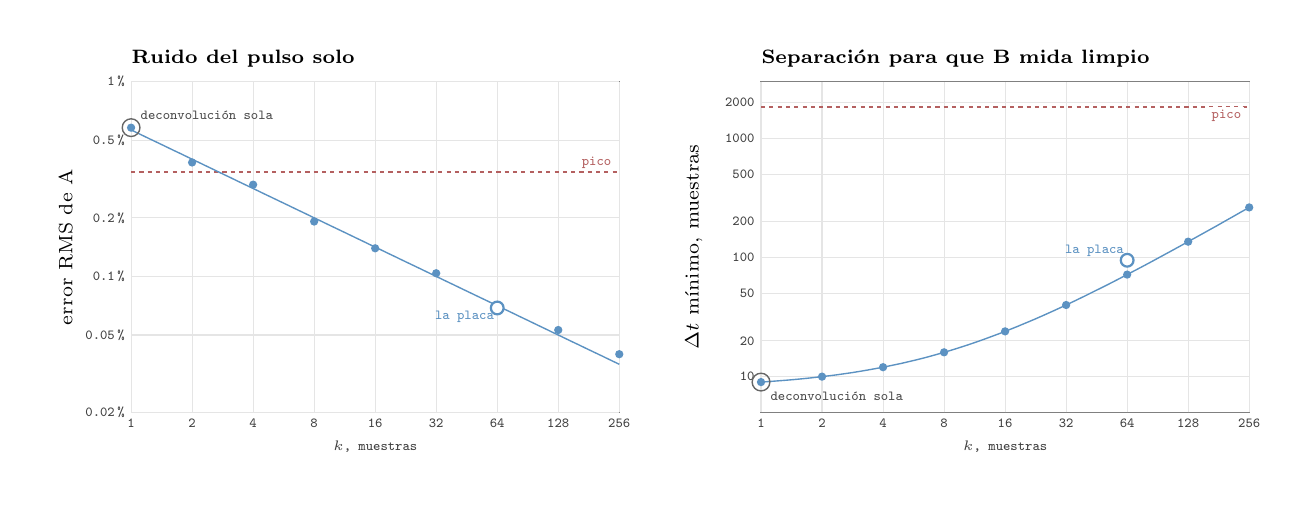
\begin{tikzpicture}[fondo]
\node[anchor=south west, font=\scriptsize\bfseries, inner sep=0pt] at (0.000,4.380) {Ruido del pulso solo};
\draw[black!50, line width=0.4pt] (0.000,0.000) rectangle (6.200,4.200);
\draw[black!10] (0.000,0.000) -- (6.200,0.000);
\node[nodo, anchor=east] at (-0.040,0.000) {0.02\,\%};
\draw[black!10] (0.000,0.984) -- (6.200,0.984);
\node[nodo, anchor=east] at (-0.040,0.984) {0.05\,\%};
\draw[black!10] (0.000,1.728) -- (6.200,1.728);
\node[nodo, anchor=east] at (-0.040,1.728) {0.1\,\%};
\draw[black!10] (0.000,2.472) -- (6.200,2.472);
\node[nodo, anchor=east] at (-0.040,2.472) {0.2\,\%};
\draw[black!10] (0.000,3.456) -- (6.200,3.456);
\node[nodo, anchor=east] at (-0.040,3.456) {0.5\,\%};
\draw[black!10] (0.000,4.200) -- (6.200,4.200);
\node[nodo, anchor=east] at (-0.040,4.200) {1\,\%};
\draw[black!10] (0.000,0.000) -- (0.000,4.200);
\node[nodo, anchor=north] at (0.000,-0.040) {1};
\draw[black!10] (0.775,0.000) -- (0.775,4.200);
\node[nodo, anchor=north] at (0.775,-0.040) {2};
\draw[black!10] (1.550,0.000) -- (1.550,4.200);
\node[nodo, anchor=north] at (1.550,-0.040) {4};
\draw[black!10] (2.325,0.000) -- (2.325,4.200);
\node[nodo, anchor=north] at (2.325,-0.040) {8};
\draw[black!10] (3.100,0.000) -- (3.100,4.200);
\node[nodo, anchor=north] at (3.100,-0.040) {16};
\draw[black!10] (3.875,0.000) -- (3.875,4.200);
\node[nodo, anchor=north] at (3.875,-0.040) {32};
\draw[black!10] (4.650,0.000) -- (4.650,4.200);
\node[nodo, anchor=north] at (4.650,-0.040) {64};
\draw[black!10] (5.425,0.000) -- (5.425,4.200);
\node[nodo, anchor=north] at (5.425,-0.040) {128};
\draw[black!10] (6.200,0.000) -- (6.200,4.200);
\node[nodo, anchor=north] at (6.200,-0.040) {256};
\node[nodo, anchor=north] at (3.100,-0.320) {$k$, muestras};
\node[font=\scriptsize, anchor=south, rotate=90] at (-0.620,2.100) {error RMS de A};
\draw[rojo!75!black, line width=0.8pt, dash pattern=on 1.5pt off 1.5pt] (0.000,3.056) -- (6.200,3.056);
\node[nodo, anchor=south east, text=rojo!75!black, fill=white, inner sep=1pt] at (6.140,3.056) {pico};
\draw[azul!85!black, line width=0.5pt] plot coordinates {(0.000,3.588) (0.105,3.538) (0.210,3.487) (0.315,3.437) (0.420,3.387) (0.525,3.336) (0.631,3.286) (0.736,3.235) (0.841,3.185) (0.946,3.134) (1.051,3.084) (1.156,3.033) (1.261,2.983) (1.366,2.932) (1.471,2.882) (1.576,2.832) (1.681,2.781) (1.786,2.731) (1.892,2.680) (1.997,2.630) (2.102,2.579) (2.207,2.529) (2.312,2.478) (2.417,2.428) (2.522,2.377) (2.627,2.327) (2.732,2.277) (2.837,2.226) (2.942,2.176) (3.047,2.125) (3.153,2.075) (3.258,2.024) (3.363,1.974) (3.468,1.923) (3.573,1.873) (3.678,1.823) (3.783,1.772) (3.888,1.722) (3.993,1.671) (4.098,1.621) (4.203,1.570) (4.308,1.520) (4.414,1.469) (4.519,1.419) (4.624,1.368) (4.729,1.318) (4.834,1.268) (4.939,1.217) (5.044,1.167) (5.149,1.116) (5.254,1.066) (5.359,1.015) (5.464,0.965) (5.569,0.914) (5.675,0.864) (5.780,0.813) (5.885,0.763) (5.990,0.713) (6.095,0.662) (6.200,0.612)};
\fill[azul!85!black] (0.000,3.617) circle (1.5pt);
\fill[azul!85!black] (0.775,3.175) circle (1.5pt);
\fill[azul!85!black] (1.550,2.893) circle (1.5pt);
\fill[azul!85!black] (2.325,2.425) circle (1.5pt);
\fill[azul!85!black] (3.100,2.085) circle (1.5pt);
\fill[azul!85!black] (3.875,1.768) circle (1.5pt);
\fill[azul!85!black] (4.650,1.328) circle (1.5pt);
\fill[azul!85!black] (5.425,1.047) circle (1.5pt);
\fill[azul!85!black] (6.200,0.740) circle (1.5pt);
\draw[azul!85!black, fill=white, line width=0.8pt] (4.650,1.327) circle (2.3pt);
\node[nodo, anchor=north east, text=azul!85!black] at (4.650,1.327) {la placa};
\draw[black!60, line width=0.5pt] (0.000,3.617) circle (3.2pt);
\node[anchor=south west, font=\scriptsize\bfseries, inner sep=0pt] at (8.000,4.380) {Separación para que B mida limpio};
\draw[black!50, line width=0.4pt] (8.000,0.000) rectangle (14.200,4.200);
\draw[black!10] (8.000,0.455) -- (14.200,0.455);
\node[nodo, anchor=east] at (7.960,0.455) {10};
\draw[black!10] (8.000,0.910) -- (14.200,0.910);
\node[nodo, anchor=east] at (7.960,0.910) {20};
\draw[black!10] (8.000,1.512) -- (14.200,1.512);
\node[nodo, anchor=east] at (7.960,1.512) {50};
\draw[black!10] (8.000,1.967) -- (14.200,1.967);
\node[nodo, anchor=east] at (7.960,1.967) {100};
\draw[black!10] (8.000,2.422) -- (14.200,2.422);
\node[nodo, anchor=east] at (7.960,2.422) {200};
\draw[black!10] (8.000,3.024) -- (14.200,3.024);
\node[nodo, anchor=east] at (7.960,3.024) {500};
\draw[black!10] (8.000,3.479) -- (14.200,3.479);
\node[nodo, anchor=east] at (7.960,3.479) {1000};
\draw[black!10] (8.000,3.934) -- (14.200,3.934);
\node[nodo, anchor=east] at (7.960,3.934) {2000};
\draw[black!10] (8.000,0.000) -- (8.000,4.200);
\node[nodo, anchor=north] at (8.000,-0.040) {1};
\draw[black!10] (8.775,0.000) -- (8.775,4.200);
\node[nodo, anchor=north] at (8.775,-0.040) {2};
\draw[black!10] (9.550,0.000) -- (9.550,4.200);
\node[nodo, anchor=north] at (9.550,-0.040) {4};
\draw[black!10] (10.325,0.000) -- (10.325,4.200);
\node[nodo, anchor=north] at (10.325,-0.040) {8};
\draw[black!10] (11.100,0.000) -- (11.100,4.200);
\node[nodo, anchor=north] at (11.100,-0.040) {16};
\draw[black!10] (11.875,0.000) -- (11.875,4.200);
\node[nodo, anchor=north] at (11.875,-0.040) {32};
\draw[black!10] (12.650,0.000) -- (12.650,4.200);
\node[nodo, anchor=north] at (12.650,-0.040) {64};
\draw[black!10] (13.425,0.000) -- (13.425,4.200);
\node[nodo, anchor=north] at (13.425,-0.040) {128};
\draw[black!10] (14.200,0.000) -- (14.200,4.200);
\node[nodo, anchor=north] at (14.200,-0.040) {256};
\node[nodo, anchor=north] at (11.100,-0.320) {$k$, muestras};
\node[font=\scriptsize, anchor=south, rotate=90] at (7.380,2.100) {$\Delta t$ mínimo, muestras};
\draw[rojo!75!black, line width=0.8pt, dash pattern=on 1.5pt off 1.5pt] (8.000,3.884) -- (14.200,3.884);
\node[nodo, anchor=north east, text=rojo!75!black, fill=white, inner sep=1pt] at (14.140,3.884) {pico};
\draw[azul!85!black, line width=0.5pt] plot coordinates {(8.000,0.386) (8.105,0.393) (8.210,0.401) (8.315,0.409) (8.420,0.418) (8.525,0.428) (8.631,0.439) (8.736,0.451) (8.841,0.463) (8.946,0.476) (9.051,0.491) (9.156,0.506) (9.261,0.523) (9.366,0.541) (9.471,0.560) (9.576,0.580) (9.681,0.602) (9.786,0.624) (9.892,0.649) (9.997,0.674) (10.102,0.701) (10.207,0.730) (10.312,0.760) (10.417,0.791) (10.522,0.824) (10.627,0.858) (10.732,0.894) (10.837,0.931) (10.942,0.970) (11.047,1.009) (11.153,1.051) (11.258,1.093) (11.363,1.137) (11.468,1.181) (11.573,1.227) (11.678,1.274) (11.783,1.322) (11.888,1.371) (11.993,1.421) (12.098,1.472) (12.203,1.524) (12.308,1.576) (12.414,1.629) (12.519,1.683) (12.624,1.738) (12.729,1.793) (12.834,1.848) (12.939,1.904) (13.044,1.961) (13.149,2.018) (13.254,2.075) (13.359,2.133) (13.464,2.191) (13.569,2.249) (13.675,2.308) (13.780,2.366) (13.885,2.426) (13.990,2.485) (14.095,2.545) (14.200,2.604)};
\fill[azul!85!black] (8.000,0.386) circle (1.5pt);
\fill[azul!85!black] (8.775,0.455) circle (1.5pt);
\fill[azul!85!black] (9.550,0.575) circle (1.5pt);
\fill[azul!85!black] (10.325,0.764) circle (1.5pt);
\fill[azul!85!black] (11.100,1.030) circle (1.5pt);
\fill[azul!85!black] (11.875,1.365) circle (1.5pt);
\fill[azul!85!black] (12.650,1.751) circle (1.5pt);
\fill[azul!85!black] (13.425,2.169) circle (1.5pt);
\fill[azul!85!black] (14.200,2.604) circle (1.5pt);
\draw[azul!85!black, fill=white, line width=0.8pt] (12.650,1.933) circle (2.3pt);
\node[nodo, anchor=south east, text=azul!85!black] at (12.650,1.933) {la placa};
\draw[black!60, line width=0.5pt] (8.000,0.386) circle (3.2pt);
\node[nodo, anchor=south west, text=black!70] at (0.080,3.677) {deconvolución sola};
\node[nodo, anchor=north west, text=black!70] at (8.080,0.306) {deconvolución sola};
\end{tikzpicture}
\end{document}
